\begin{enumerate}
	\item From 
		\eqref{prop:lin-eq-unit-mat},
\begin{align}
\myvec{1&6&-4\\1&4&-2\\-1&-5&3}^\top \vec{n}=\myvec{1\\1\\1}
\implies \myvec{1&1&-1\\ 6&4&-5\\ -4&-2&3} \vec{n} = \myvec{1\\1\\1}
\end{align}
the augmented matrix is given by,
\begin{align}
\myvec{1&1&-1&\vrule&1\\6&4&-5&\vrule&1\\-4&-2&3&\vrule&1}
\xleftrightarrow[R_3 \leftarrow R_3 + 4R_1]{R_2 \leftarrow R_2 - 6R_1}
\myvec{1&1&-1&\vrule&1\\0&-2&1&\vrule&-5\\0&2&-1&\vrule&5}\\ 
\xleftrightarrow{R_2 \leftarrow \frac{-R_2}{2}} 
\myvec{1&1&-1&\vrule&1\\0&1&\frac{-1}{2}&\vrule&\frac{5}{2}\\0&2&-1&\vrule&5}
\xleftrightarrow[{R_1 \leftarrow R_1 - R_2}] {R_3 \leftarrow R_3 - 2R_2}
\myvec{1&0&\frac{-1}{2}&\vrule&\frac{-3}{2}\\0&1&\frac{-1}{2}&\vrule&\frac{5}{2}\\0&0&0&\vrule&0}
\end{align}
Since we obtain a 0 row, 
the given points are collinear.
The direction vector of the line is
\begin{align}
\vec{m}=\vec{B}-\vec{C} = \myvec{10\\6\\-8}
\end{align}
and the equation of a line is given by,
\begin{align}
	\vec{x}&=\vec{p}+  \lambda \vec{m}\\
	\implies \vec{x}&= \myvec{1\\1\\– 1} + \lambda \myvec{10\\6\\-8}
\end{align}
See 
     \figref{fig:chapters/12/11/3/6/1}.
\begin{figure}[h!]
  \centering
   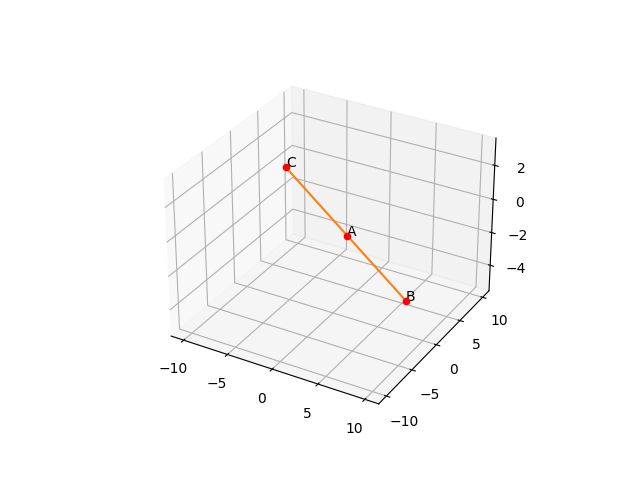
\includegraphics[width=\columnwidth]{chapters/12/11/3/6/figs/collinear_points.png}
    \caption{The figure shows that the given points are collinear}
     \label{fig:chapters/12/11/3/6/1}
     \end{figure}
     \item  In this case, 
\begin{align}
\myvec{1&1&-2\\1&2&2\\0&1&-1}^\top \vec{n}=\vec{1}
\implies \myvec{1&1&0 \\ 1&2&1 \\ -2&2&-1} \vec{n}=\vec{1}
\end{align}
The augmented matrix is given by,
\begin{align}
\myvec{1&1&0&\vrule&1\\1&2&1&\vrule&1\\-2&2&-1&\vrule&1}
\xleftrightarrow[R_3 \leftarrow R_3 + 2R_1]{R_2 \leftarrow R_2 - R_1}
\myvec{1&1&0&\vrule&1\\0&1&1&\vrule&0\\0&4&-1&\vrule&3}\\
\xleftrightarrow{R_1 \leftarrow R_1- R_2}
\myvec{1&0&-1&\vrule&1\\0&1&1&\vrule&0\\0&4&-1&\vrule&3}
\xleftrightarrow{R_3 \leftarrow R_3 - 4R_2}
\myvec{1&0&-1&\vrule&1\\0&1&1&\vrule&0\\0&0&-5&\vrule&3}\\
\xleftrightarrow{R_3 \leftarrow \frac{- R_3}{5}}
\myvec{1&0&-1&\vrule&1\\0&1&1&\vrule&0\\0&0&1&\vrule&\frac{-3}{5}}
\xleftrightarrow[R_1 \leftarrow R_1 + R_3]{R_2 \leftarrow R_2 - R_3}
\myvec{1&0&0& \vrule& \frac{2}{5}  \\ 0&1&0& \vrule& \frac{3}{5} \\ 0&0&1& \vrule& \frac{-3}{5}}
\end{align}
Hence, the equation of the plane is
\begin{align}
\myvec{2 & 3 & -3} \vec{x} = 5
\end{align}
See 
     \figref{fig:chapters/12/11/3/6/2}
\begin{figure}[h!]
  \centering
   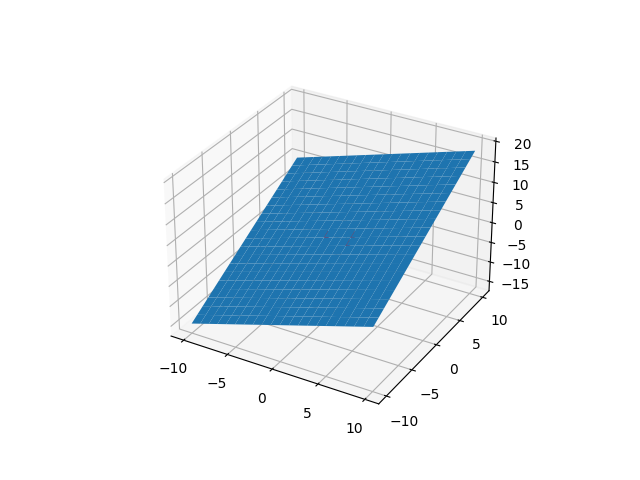
\includegraphics[width=\columnwidth]{chapters/12/11/3/6/figs/plane_b.png}
    \caption{Plane passing through the given points }
     \label{fig:chapters/12/11/3/6/2}
     \end{figure} 
\end{enumerate}
